\begin{figure*}[!htpb]
	\centering
	\begin{subfigure}{1.0\textwidth}
		\centering
		\caption{}
		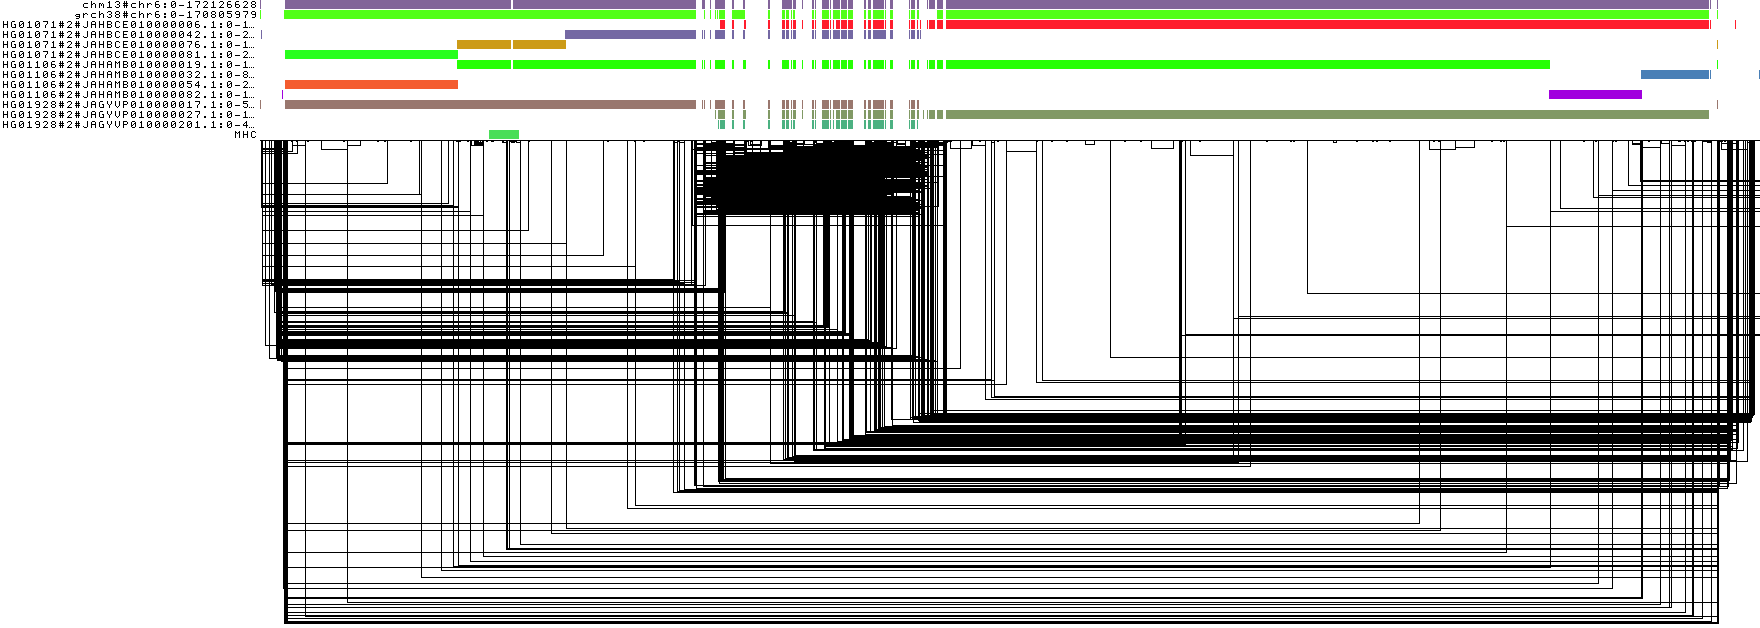
\includegraphics[width=1.0\linewidth]{fig/1D/chr6.hprc-v1.0-pggb.13paths.MHC.og.png}
		\label{fig:1d_fig1}
	\end{subfigure}
	\\
	\begin{subfigure}{1.0\textwidth}
		\centering
		\caption{}
		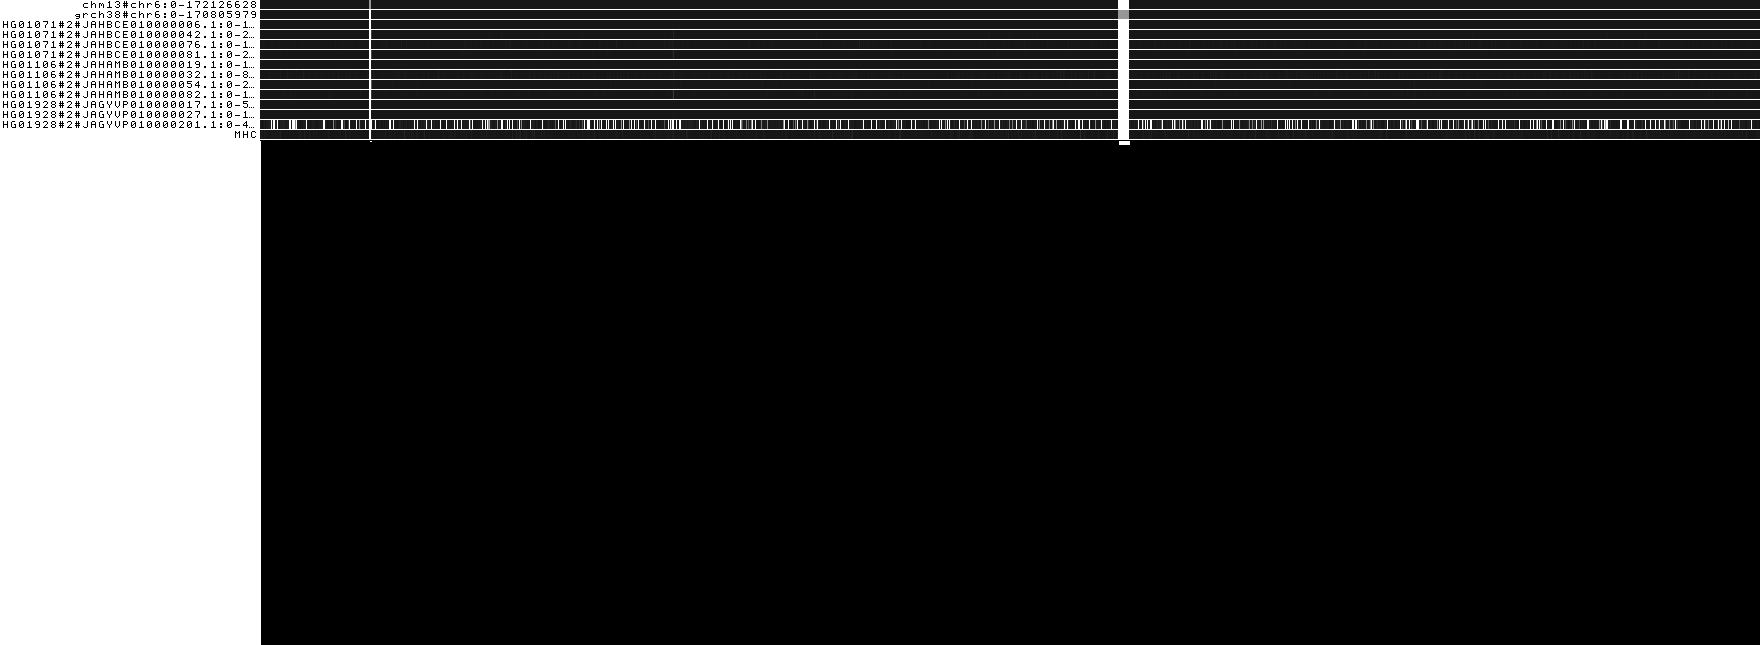
\includegraphics[width=1.0\linewidth]{fig/1D/chr6.hprc-v1.0-pggb.13paths.MHC.og.r.og.png}
		\label{fig:1d_fig2}
	\end{subfigure}
	\\
	\begin{subfigure}{1.0\textwidth}
		\centering
		\caption{}
		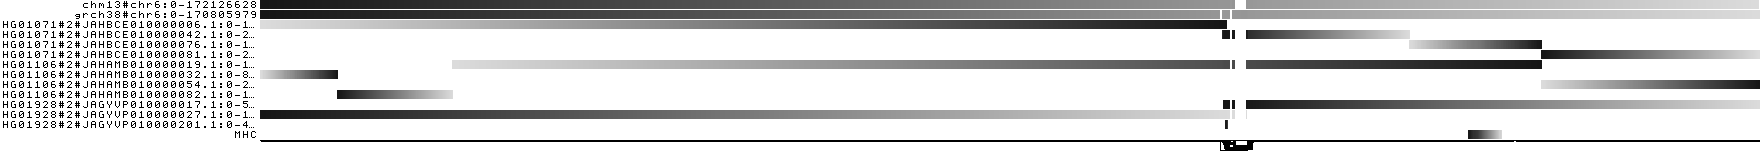
\includegraphics[width=1.0\linewidth]{fig/1D/chr6.hprc-v1.0-pggb.13paths.MHC.og.r.og.Y.og.png}
		\label{fig:1d_fig3}
	\end{subfigure}
	\\
	\begin{subfigure}{1.0\textwidth}
		\centering
		\caption{}
		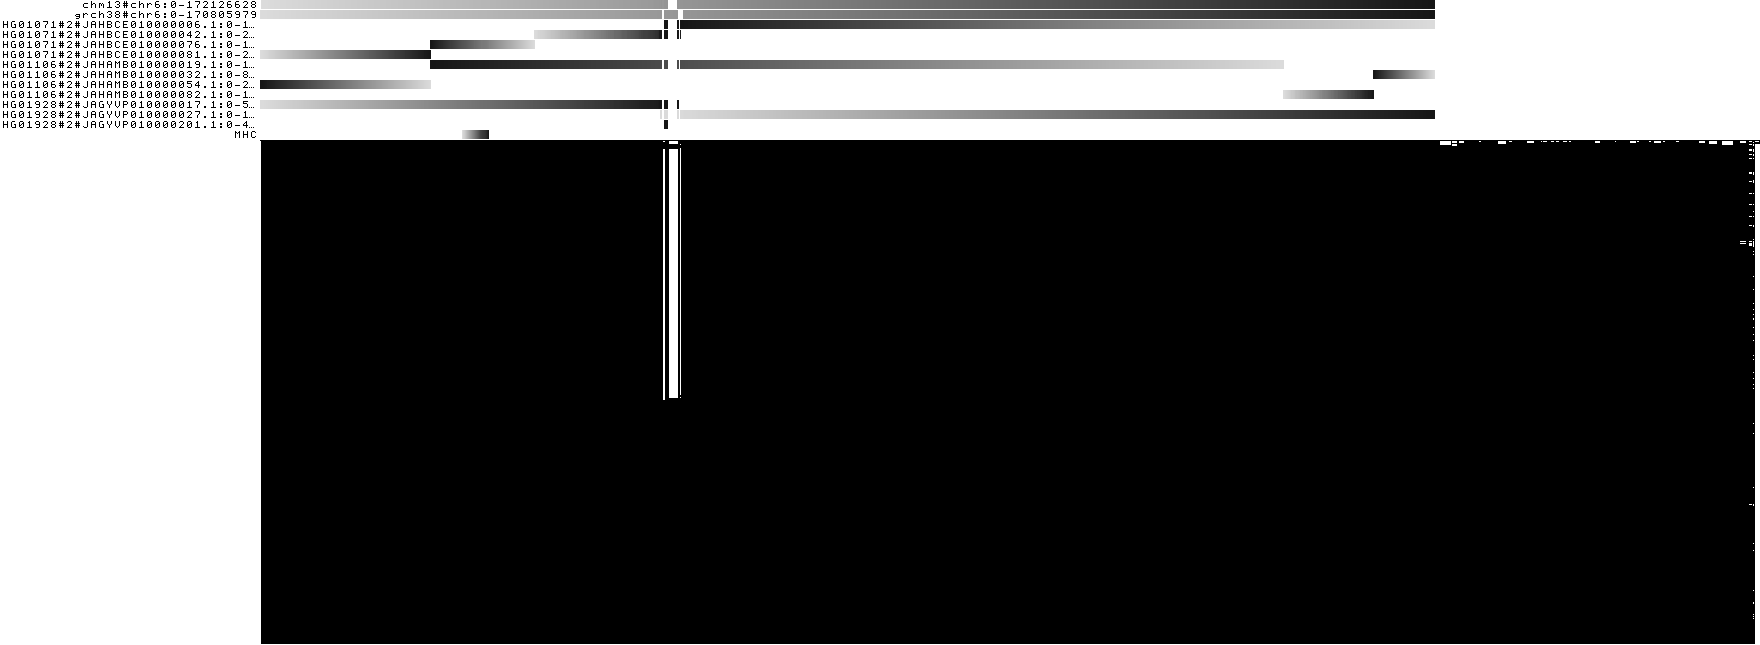
\includegraphics[width=1.0\linewidth]{fig/1D/chr6.hprc-v1.0-pggb.13paths.MHC.og.r.og.HY.og.png}
		\label{fig:1d_fig4}
	\end{subfigure}	
	\caption{\textit{odgi viz} 1D visualizations of a 5 haplotypes subgraph of the Human Pangenome Resource Consortium (HPRC) chromosome 6 pangenome graph. The major histocompatibility complex (MHC) sequence was injected as an extra path. Various node arrangements are shown. 
		\textbf{a-d} A graphs nodes are arranged from left to right forming the pangenome sequence. The black lines under the paths are the links representing the topology. Path names are left.
		\textbf{(a)} \textit{odgi viz} default modality: The colored bars are the paths versus pangenome sequence in a binary matrix. Shown is the subgraph extracted with \textit{odgi extract}. No 1D layout algorithm was applied here.
		\textbf{b-d} \textit{odgi viz} colored by path position. Light grey corresponds to the beginning of a path, black encodes the end of the path.
		\textbf{(b)} The nodes are arranged randomly in 1D.
		\textbf{(c)} The nodes are arranged applying the 1D PG-SGD algorithm.
		\textbf{(d)} The nodes are arranged applying a 1D reference-guided PG-SGD where the nodes of haplotype HG01071 are fixed and only all the othere ones are movable in 1D. Now all paths of this haplotype are arranged from their lowest to their highest nucleotide position. However,lot's of longer links are now visible compared to the node ordering directly above. This indicates a node order that is globally not optimal.}
	\label{fig:1d_sorts}
\end{figure*}